\documentclass[dvipdfmx,autodetect-engine,titlepage]{jsarticle}
\usepackage[dvipdfm]{graphicx}
\usepackage{ascmac}
\usepackage{fancybox}
\usepackage{listings}
\usepackage{plistings}
\usepackage{itembkbx}
\usepackage{amsmath}
\usepackage{url}
\usepackage{graphics}
\usepackage{listings}
\usepackage{here}

\lstset{%
  language={C},
  basicstyle={\small},%
  identifierstyle={\small},%
  commentstyle={\small\itshape\color[rgb]{0,0.5,0}},%
  keywordstyle={\small\bfseries\color[rgb]{0,0,1}},%
  ndkeywordstyle={\small},%
  stringstyle={\small\ttfamily\color[rgb]{1,0,1}},
  frame={tb},
  breaklines=true,
  columns=[l]{fullflexible},%
  numbers=left,%
  xrightmargin=0zw,%
  xleftmargin=3zw,%
  numberstyle={\scriptsize},%
  stepnumber=1,
  numbersep=1zw,%
  lineskip=-0.5ex%
}

\textheight=23cm
\renewcommand{\figurename}{図}
\renewcommand{\tablename}{表}
\newenvironment{code}
{\vspace{0.5zw}\VerbatimEnvironment  \begin{screen} 
\baselineskip=1.0\normalbaselineskip
 \begin{Verbatim}}
{\end{Verbatim}
\baselineskip=\normalbaselineskip
 \end{screen}\vspace{0.5zw}} 

\title{セキュリティ・ネットワーク学実験3(B2)\\
アプリケーション脆弱性実習レポート\\
}
\author{2600200087-2\\Oku Wakana\\奥 若菜}
\date{Jun.29 2022}

\begin{document}

\maketitle

\section{問1 アーカイブソフトの異常終了(1)}
\subsection{スタック領域におけるバッファオーバーフロー}
外部からの入力によって確保したバッファ以上のデータがプログラムに読み込まれ、それが変数にコピーされることで、コピー先のバッファからデータが溢れ、隣の変数の内容が上書きされてしまうことがある。このような現象をバッファオーバーフローという。
ここでは、脆弱アーカイブソフトに含まれるスタック領域におけるバッファオーバーフローの脆弱性を確認する。\\
\subsection{演習1/9}
脆弱アーカイブソフトを使ってArchiverSample.zipを展開し、その様子をキャプチャした。図1のようにファイルを展開したところ、動作が完了し、図2のようにsample.txtという名前のファイルが作成された。\\

\begin{figure}[H]
  \centering
  \begin{minipage}[b]{0.45\linewidth}
  \begin{center}
    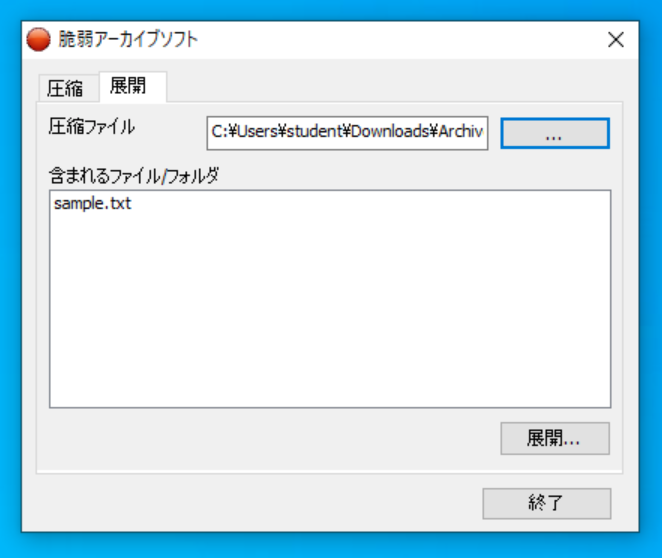
\includegraphics[keepaspectratio,scale=0.6]{fg1.png}
    \end{center}
    \caption{ファイル展開}
  \end{minipage}
  \begin{minipage}[b]{0.45\linewidth}
  \begin{center}
    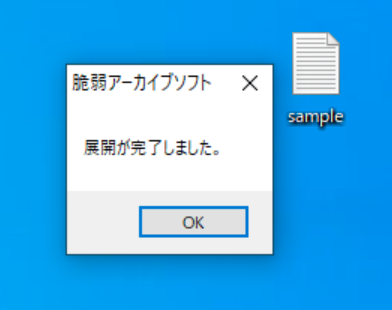
\includegraphics[keepaspectratio,scale=0.8]{fg2.png}
    \end{center}
    \caption{展開完了}
  \end{minipage}
\end{figure}

 \\\\
\subsection{演習3/9}
脆弱アーカイブソフトを使ってArchiverCheckBOF.zipを展開し、その様子をキャプチャした。図2のようにファイルを展開しようとしたところ、図4のように、脆弱アーカイブソフトが異常終了し、zipファイルを展開することはできなかった。
これは、zipファイルに含まれるファイルまたはフォルダ名が、あらかじめ確保したバッファ以上の長さだったため、バッファオーバーフローが起きたことよって、異常終了したと考えられる。

\begin{figure}[H]
  \centering
  \begin{minipage}[b]{0.45\linewidth}
  \begin{center}
    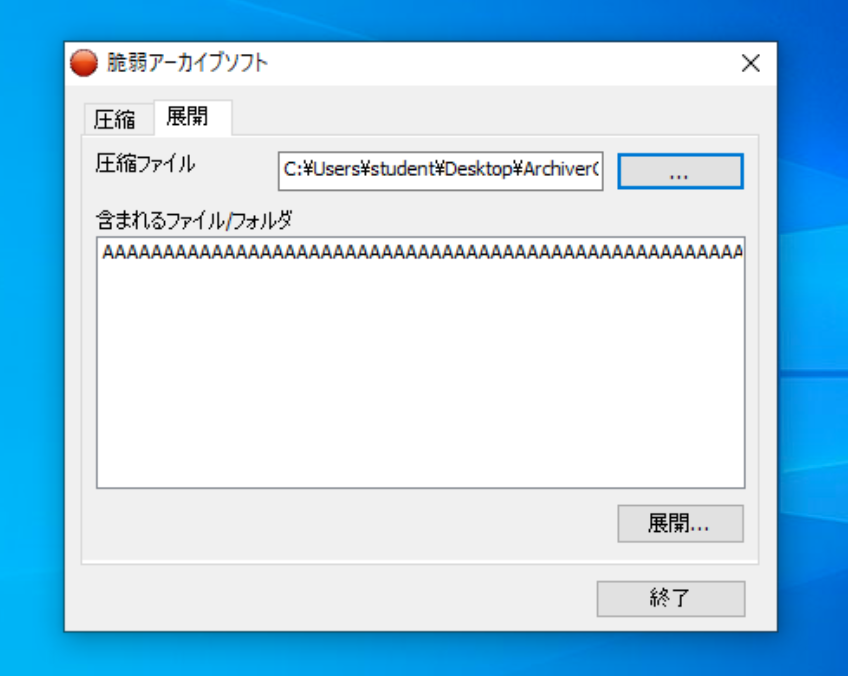
\includegraphics[keepaspectratio,scale=0.5]{fg3.png}
    \end{center}
    \caption{ファイル展開}
  \end{minipage}
  \begin{minipage}[b]{0.45\linewidth}
  \begin{center}
    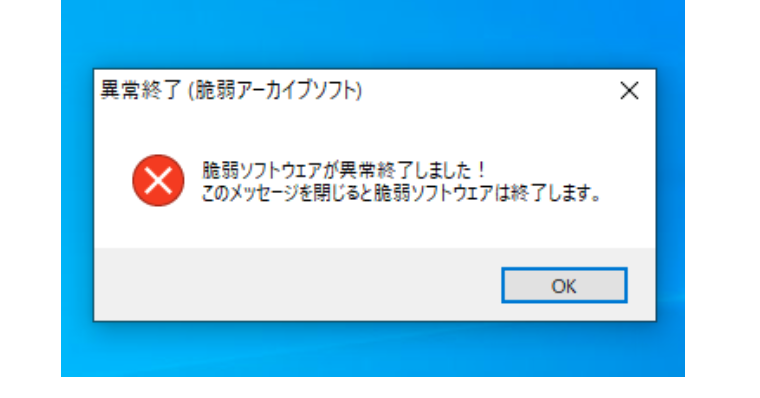
\includegraphics[keepaspectratio,scale=0.6]{fg4.png}
    \end{center}
    \caption{異常終了}
  \end{minipage}
\end{figure}

\section{問2 アーカイブソフトの異常終了(2)}
\subsection{演習4/9}
脆弱アーカイブソフトを使って、擬似攻撃ファイルArchiverAttackBOF.zipを展開し、その様子をキャプチャした。
脆弱性が悪用されることにより、ダイアログを表示させるマシンコードが実行された結果、下の図5のようなダイアログが表示された。
演習3/9との違いとして、プログラムが異常終了した結果、ダイアログが表示されたのではなく、マシンコードによって表示されたものであるという点が挙げられる。\\
\begin{figure}[H]
  \centering
  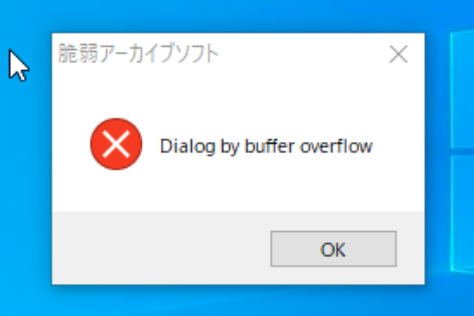
\includegraphics[scale=0.8]{fg5.png}
  \caption{実行結果}\label{fig:図5}
\end{figure}

\subsection{問2.1}
バッファオーバーフローが起きた際に、プログラムが異常終了する理由は、UNIX系のOS上では、不正なメモリにアクセスするプロセスはSIGSEGシグナルを受けとるためである。
これにより、プロセスがOSによって止められ、異常終了したと考えられる。また、他のOSを利用する場合も同様に例外を受け取る。
プログラムの表示がおかしくなったり、変数値がおかしくなったりする理由としては、バッファオーバーフローによって、溢れたデータで他のメモリ内容が上書きされ、変数の値が書き換えられるためと考えられる。

\subsection{問2.2}
攻撃者によって、任意のプログラムが送り込まれる方法と、そのプログラムが実行される原理を説明する。攻撃者は、スタックオーバーフローを用いて、任意のマシンコードをメモリ上に書き込む。そして関数のreturnアドレスを、そのマシンコードが書かれた先頭アドレスに書き換えることで、任意のプログラムを実行させる。\\



\subsection{問2.3}
フォーマット文字列を用いた攻撃では、フォーマット文字列として\%nが最も危険だといわれている。この\%nを用いた攻撃の原理を説明する。\%nは、これまでの書式編集出力で何バイトのデータが書き出されたかの値を整数変数に書き戻すことを指示する書式である。これを使い、ポインタ変数の値を任意のアドレスに書き換えることで、実行したいマシンコードの先頭アドレスに飛ばすことができる。\\

\section{問3 脆弱Archiverの修正}
1,2章で確認した脆弱性を、ソースコードを修正することで、異常終了が起こらないようにする。脆弱性の原因は、圧縮されたファイル内のファイル名のコピーに、strcpy関数を使っているためだと考えられる。これをstrncpy関数に置き換え、コピーする文字列の長さを制限することで、バッファオーバーフローが起こることを防ぐ。\\\\
下の図6は、修正をおこなった後にArchiverCheckBOF.zipを展開した結果である。異常終了することは無くなったが、別のエラーが発生し、ファイルを作成することはできなかった。\\
\begin{figure}[H]
  \centering
  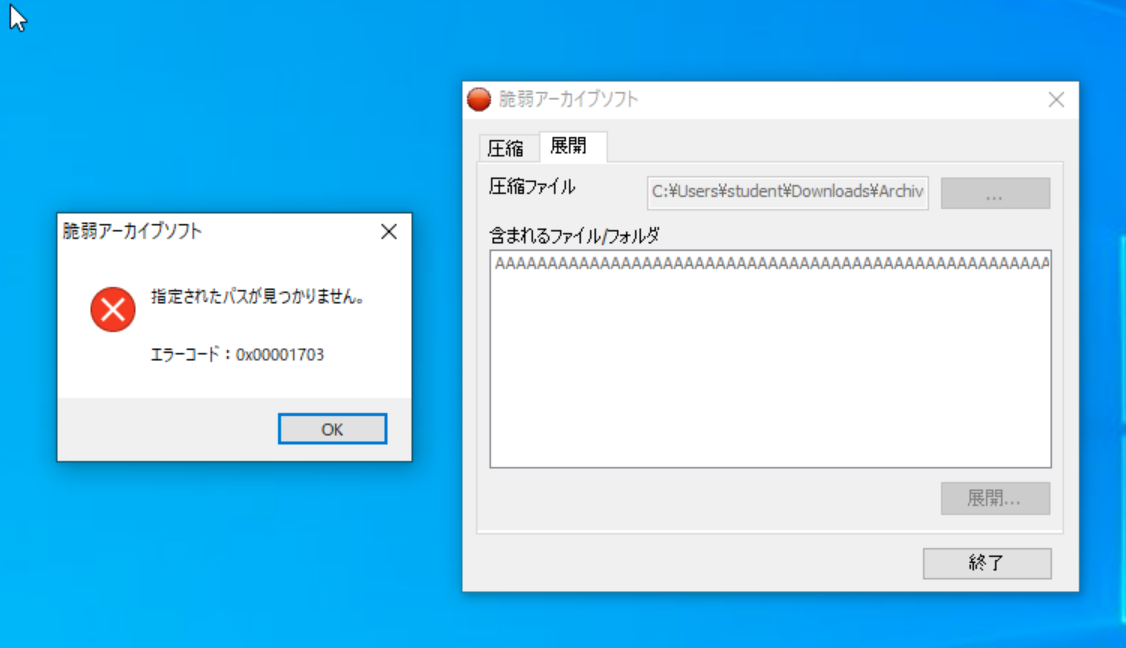
\includegraphics[scale=0.6]{fg8.png}
  \caption{実行結果}\label{fig:図8}
\end{figure}



\section{問4 整数オーバーフロー}

\subsection{演習3/7}
脆弱アーカイブソフトを使って、ArchiverCheckIOF.zipを展開したところ、整数オーバーフロー脆弱性がバッファオーバーフローを誘発し、下の図7のようにプログラムが異常終了した。\\
\begin{figure}[H]
  \centering
  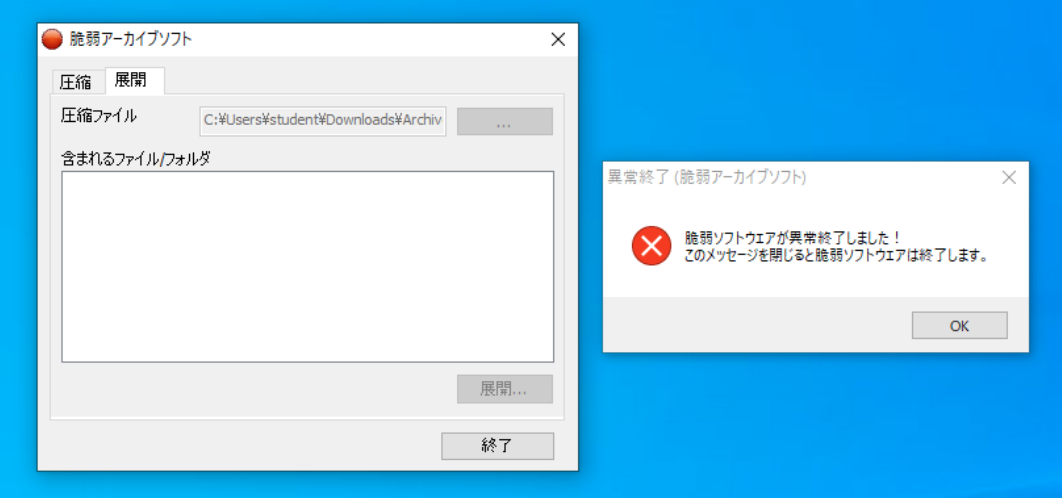
\includegraphics[scale=0.6]{fg6.png}
  \caption{実行結果}\label{fig:図6}
\end{figure}

\subsection{演習4/7}
脆弱アーカイブソフトを使って、擬似攻撃ファイルArchiverAttackIOF.zipを展開し、その様子をキャプチャした。
整数オーバーフロー脆弱性が悪用されることにより、バッファオーバーフローが誘発され、ダイアログを表示させるマシンコードが実行された結果、下の図8のようなダイアログが表示された。
演習3/7との違いとして、プログラムが異常終了した結果、ダイアログが表示されたのではなく、マシンコードによって表示されたものであるという点が挙げられる。\\

\begin{figure}[H]
  \centering
  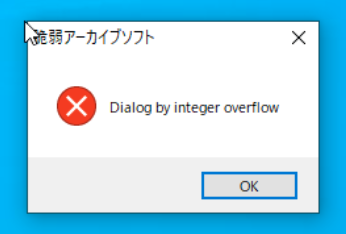
\includegraphics[scale=0.9]{fg7.png}
  \caption{実行結果}\label{fig:図7}
\end{figure}


\end{document}
